\newpage
% Principe de codage 100 sign (rapport et code de guy)?

\section{Plate-forme de tests}

Pour évaluer la performance de carte acoustique Version 4G, j'ai conçu une procédure de test qui est divisé en trois phases:\\

\noindent\textbf{Phase 1:} Plan du test\\
\textbf{Phase 2:} Démarrage du test\\
\textbf{Phase 3:} Analyse des résultats
%%%%%%%%%%%%%%%%%%%%%%%%%%%%%%%%%%%%%%%%%%%%%%%%%%%%%%%%%%%%%%%%%%%%%%%%%%%%%%%%%%%%%%%%%%%%%%%%%%%%%%%%%%%%%%%%%%%%%%%%%%%%%%%%%%%%%%%%%%%%
\subsection{Phase 1: Plan du test}

\textbf{TEST 1: Fiabilité de l'encryptage}\\
Objectifs du test:Valider les éléments constituants d'une trame acoustique et le taux de récupération.\\

\textbf{TEST 2: Fiabilité émission sonore}\\
Objectifs du test:Observer la génération de signaux harmoniques lors de l'émission de la trame acoustique et vérifier que ceux-ci sont identiques avec les signaux harmoniques générés par la trame de référence.\\

\textbf{TEST 3: Consommation}\\
Objectifs du test:S'assurer que la consommation par le prototype est conforme à la consommation attendue.\\

\textbf{TEST 4: Durée de vie}\\
Objectifs du test:Obtenir, dans le plus mauvais des cas (utilisation continue, sans endormissement), le nombre d'utilisations possibles pour une pile SoliCore 10mAh.\\

\textbf{TEST 5: Récupération via IPad}\\
Objectifs du test:Observer les taux de récupération des trames sur un équipement de type IPad.\\

\textbf{TEST 6: Récupération via IPhone}\\
Objectifs du test:Observer les taux de récupération des trames sur un équipement de type IPhone.\\

\textbf{TEST 7: Récupération via Windows}\\
Objectifs du test:Observer les taux de récupération des trames sur un équipement de type ordinateur portable.\\

Pour certain test, il y a des facteurs à considérer (Pour obtenir le pourcentage de récupération par exemple):

\subsubsection{Distances}
Pour chaque test, il y a 4 conditions de distance, marqué par C, N, B, S. qui sont resspectivement les acronymes de Contact, Near, Beside, Speakerphone:\\

\begin{itemize}
\item \textbf{C}ontact: La carte doit être utilisée collée, plaquée ou appliquée contre le combiné, téléphone portable en contact physique avec le terminal.
\item \textbf{N}ear: La carte doit être utilisée proche du combiné du téléphone entre trois et quatre centimètress, assez proche du microphone. Cette distance corresspondant approximativement à l'épaisseur de deux doigts.
\item \textbf{B}eside: La carte doit être utilisée à dix centimètress du combiné du téléphone. Cette distance corresspondant approximativement à la largeur d'une main.
\item \textbf{S}peakerphone: Le mode haut-parleur ou main libre doit être activé en début de communication. La carte doit être utilisée à quelques centimètress du combiné du téléphone. Cette distance peut être très variable en fonction de votre configuration. Vous pouvez indiquer des détails dans le champ Phone Brand Model.\\
\end{itemize}

\subsubsection{Importance}
Le niveau d'importance de chaque test:
\begin{itemize}
\item \textbf{1:} Pas importante
\item \textbf{2:} Importante
\item \textbf{3:} Critique
\item \textbf{4:} Vital pour la mesure de reconnaissance
\end{itemize}

\subsubsection{Périphériques}
Liste de périphériques:
\begin{itemize}
\item Mobile iPhone4
\item Mobile iPhone4s
\item Mobile iPhone5
\item Tablette iPad2
\item Tablette iPad3
\item Tablette iPad4
\item PC desktop avec microphone externe
\item PC laptop avec microphone interne
\item PC laptop avec microphone externe
\item SVI
\item Casque GN Netcom 2000 Stereo USB
\item Webcam Logitech Pro 9000, utilisation en mode webcam fixe
\item Téléphone Microsoft 1106 Catalina, utilisation en combiné ou haut-parleur
\end{itemize}

\subsubsection{Environnements}
Liste des environnements à tester:
\begin{itemize}
\item Calme,
\item Bruyant à définir probablement Radio source musicale, ou Radio source Vocale,
\item Bruit blanc ou Bruit Rose.
\end{itemize}

\subsubsection{Versions}
Il pourra être considéré plusieurs versions pour les périphériques, notamment version de système d'exploitation et de périphérique iPad 3 vs. iPad 4 et Windows 7 vs. Windows 8.

\subsubsection{Phases}
Pour le test de performance, il y a 2 phases:\\

\textbf{Mode Prototype:} les tests seront faits avec un montage prototype. Le prototype génère une séquence de 100 messages acoustiques dans la version à tester: 4G, version 0 ou version 1. Le prototype de ce test produit une séquence continue de 100 messages acoustiques séparé entre eux d'une durée intervalle d'une ou trois fois la durée utile du message acoustique. Pour la 4G, l'intervalle sera donc d'environ 1 ou 3 secondes, pour la V0 l'intervalle sera d'environ 880 ms ou 2,64 secondes. Une documentation de signature de la carte est disponible en Annexe \ref{sign}.\\

Il faut donc trois prototypes par version de message acoustique:
\begin{itemize}
\item intervalle = 1d = 1,25s
\item intervalle = 3d = 3.75s
\item intervalle = 1d = 1,25s avec buzzer de 20 mm avec la résonnance de 4KHz\\
\end{itemize}

\textbf{Mode Carte:} les tests seront effectués avec une carte physique vraie. Le testeur utilisera une seule carte pour tous ses tests. Par contre, il sera nécessaire de fournir une carte par version de message acoutique. Il y aura donc au moins trois cartes acoustiques s'il n'y a qu'une seule version pour la V1.

\subsubsection{Nombre de tests}
\noindent\textit{Phase Prototype: } 100 signaturess * 20 fois le test\\
\textit{Phase Carte: } 10 signaturess * 4 fois le test

\subsubsection{Logiciel utilisé}
\noindent\textit{LAMW: }LAMW est l'acronyme du logiciel ListenAcousticMessage sous Windows proposé par UINT, il a pour objectif de décoder le message acoustique généré par le prototype ou la carte.\\
\noindent\textit{LAMI: }LAMI est l'application qui est utilisée dans l'environnement IOS, avec  les mêmes fonctionnalités que LAMW.

\subsubsection{Numérotation des tests}
\noindent On utilise un tableau Excel pour lister touts les tests à faire avec leurs niveaux d'importance.

%%%%%%%%%%%%%%%%%%%%%%%%%%%%%%%%%%%%%%%%%%%%%%%%%%%%%%%%%%%%%%%%%%%%%%%%%%%%%%%%%%%%%%%%%%%%%%%%%%%%%%%%%%%%%%%%%%%%%%%%%%%%%%%%%%%%%%%%%%%%
\subsection{Phase 2: Démarrage du test}

\subsubsection{TEST 1: Fiabilité de l'encryptage}
\paragraph{Description du test: }Génération de 100 signaturess acoustiques. Les trames sont enregistrées via le programme ListenAcousticMessage v.1.2.1.71. On analyse les résultats du premier fichier (sur les 10), en comparant les OTP (a et b) récupérés avec ceux générés par le programme Display HOTP v.1.02. Une fois le premier fichier validé, on réalise une comparaison 1 à 1 (avec le premier fichier comme référence) avec le programme WinMerge v.2.14. 

\subsubsection{TEST 2: Fiabilité émission sonore}
\paragraph{Description du test: }Génération d'une trame acoustique. Enregistrement de la trame sur WaveSurfer (fréquence échantillonnage 48 KHz) et comparaison avec une trame de référence (en utilisant la version V.40 Assembleur). 

\subsubsection{TEST 3: Consommation}
\paragraph{Description du test: }Analyse de la consommation lors des différentes étapes de l'émission d'une trame acoustique. On s'assure que la consommation n'est de l'ordre du 10mA que lorsque l'on calcule, émet la trame acoustique et que l'on trouve une consommation de l'ordre de 0,1 uA lorsque le microcontrôleur est en mode «sleep». On branche le multimètre en série, entre l'alimentation (3V) et la pin Vdd du microcontrôleur. 

\subsubsection{TEST 4: Durée de vie}
\paragraph{Description du test: }Exécution continue l'émission de la trame acoustique (environ toutes les 2 secondes) jusqu'à épuisement de la pile. L'endormissement du microprocesseur et son réveil suite à l'appui sur bouton ont été tronqué. Une pile SoliCore 10mAh a été montée sur le prototype à la place des piles plates usuelles. 

\subsubsection{TEST 5: Récupération via Ipad}
\paragraph{Description du test: }Génération de 100 signaturess acoustiques. On utilise l'application smarphone UINT pour enregistrer les trames. A la fin du test, on récupère directement via l'application le nombre de trames enregistrées. On ne vérifie pas la validité des OTPs, ni de l'ID.

\paragraph{Le scénario de test}
Vous disposez un prototype du montage, avec des programmes qui fabrique un certain nombress de signaturess pour ces mesuress.\\
Par exemple, on définis 100 signaturess émis à la fois par le prototype de montage, et on enregistre les trames récupérés, puis on note le pourcentage de récupération. On répète la même opération 20 fois.\\

Il a été défini quatre positions ou distances différentes d'utilisation de la carte acoustique. vous devez suivre le déroulement pour chacune des quatre positions ou distances différentes.\\

Vous devez suivre le déroulement en gardant toujours la même distance pour une position ou distance choisie au début d'un déroulement.
Il n'est pas nécessaire de faire les séries de  déroulements en chaîne, vous pouvez les faire quand cela vous convient et dans l'ordre qu'il vous convient.

\subsubsection{TEST 6: Récupération via Iphone}
\paragraph{Description du test: }Génération de 100 signaturess acoustiques. On utilise l'application smarphone UINT pour enregistrer les trames. A la fin du test, on récupère directement via l'application le nombre de trames enregistrées. On ne vérifie pas la validité des OTPs, ni de l'ID.

\subsubsection{TEST 7: Récupération via Windows}
\paragraph{Description du test: }Génération de 100 signaturess acoustiques. On utilise l'application smarphone UINT pour enregistrer les trames. A la fin du test, on récupère directement via l'application le nombre de trames enregistrées. On ne vérifie pas la validité des OTPs, ni de l'ID.
%%%%%%%%%%%%%%%%%%%%%%%%%%%%%%%%%%%%%%%%%%%%%%%%%%%%%%%%%%%%%%%%%%%%%%%%%%%%%%%%%%%%%%%%%%%%%%%%%%%%%%%%%%%%%%%%%%%%%%%%%%%%%%%%%%%%%%%%%%%%
\subsection{Phase 3: Analyse des résultats}

\subsubsection{TEST 1: Fiabilité de l'encryptage}
Cette série de tests a permis de découvrir la non-détection d'un dépassement de taille de l'ID. En effet, l'ID est actuellement codé sous la forme de 4 octets (soit 32 bits) en mémoire Flash, mais uniquement 29 bits sont utilisés lors de la transmission du message. Si l'ID écrit en mémoire Flash à une valeur supérieure à la valeur maximale qu'il est possible de coder sur 29 bits, cela génère des erreurs lors de la génération des OTPs.\\

Pour parer à ce type d'erreur, un masque a été ajouté lors de la récupération du byte de poids fort de l'ID, pour tronquer sa valeur et bien avoir uniquement un ID sur 29 bits.

\subsubsection{TEST 2: Fiabilité émission sonore}
A l'observation sur WaveSurfer, les trames semblent similairess. On remarque que les fréquences et leurs harmoniques sont sensiblement identiques entre la trame de référence et celle étudiée. Néanmoins, en l'absence d'un outil adapté et de par le procédé d'acquisition et d'enregistrement des trames, il est difficile de faire une interprétation précise des résultats. Il convient donc de modérer le résultat de ce test. En effet, si rien ne semble «aberrant» lors de la comparaison des trames, on ne peut affirmer catégoriquement que les fréquences et harmoniques émises sont identiques.

\subsubsection{TEST 3: Consommation}
On observe bien une chute du courant consommé par le microcontrôleur lors de son entrée dans le mode «sleep». On a vérifié que le code «disassembly» de la version C est identique à la version Assembleur pour l'entrée en mode «sleep» (set GIE, set INTE, sleep).\\

Les causes de cette décroissance plus lente demandent à être investiguées plus en profondeur:
\begin{itemize}
\item Utiliser un appareil de mesure plus précis pour s'assurer qu'en mode «sleep», le microcontrôleur à la même consommation avec la V.4G en C et la V.4G en Assembleur
\item Obtenir des courbes de courant selon l'utilisation du microcontrôleur
\end{itemize}


\subsubsection{Traitement statistique des résultats}

Dès qu'on reçoit les pourcentages de Trames récupérées, on fait le traitement statistiques des résultats, par exemple:
\begin{itemize}
\item Moyenne du taux de recouvrement:M
\item Variance:V
\item Écart type des taux de recouvrement:v
\end{itemize}
On pourra également supposer que les valeurs soient normalement distribuées, cela nécessite de calculer
\begin{itemize}
\item 68\% des tests auront entre M-v et M+v de trames récupérées.
\item 95\% des tests auront entre M-2*v et M+2*v de trames récupérées.
\item 99\% des tests auront entre M-3*v et M+3*v de trames récupérées.
\end{itemize}
On pourrait alors affirmer que dans le pire des cas, le pourcentage de récupération par un périphérique dans un environnement.


\subsubsection{Analyse de l'effet filtrage sous PC}

On a fait une comparation pour voir l'effect de filtrage sous PC. Nous avons constaté que la configuration du périphérique d'enregistrement est très importante. En effet les résultats pouvaient être très variable pour une même configuration PC. On a fait donc une analyse spectrale des trames enregistrées pour chercher la raison.\\

D'abord, en Windows 8, on récupère les messages dans différentes configurations avec logiciel \texttt{wavesurfer}\footnote{Site officiel:\url{http://www.speech.kth.se/wavesurfer/}}, comme figuré ci-dessous:\\

\begin{center}
\begin{tabular}{c c}
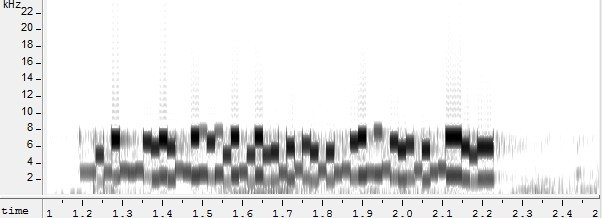
\includegraphics[scale=0.5]{images/windows8filtre} & 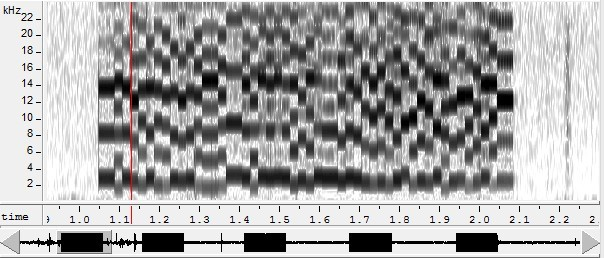
\includegraphics[scale=0.5]{images/windows8Unfiltre} \\
Avec filtrage & Sans filtrage
\end{tabular}
\end{center}

On peut voir que le filtrage coupe les fréquences qui sont supérieur à 8kHz, c'est pourquoi le résultat est trop mauvais si on utilise le filtrage du périphérique.\\

Plus précisement, la configuration est celui "Déactiver les effets de système":

\begin{center}
\begin{tabular}{c c}
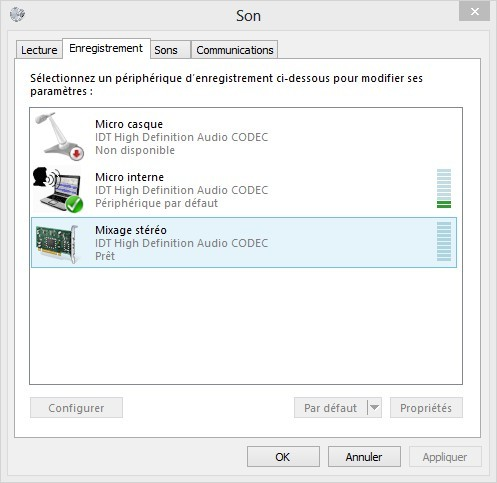
\includegraphics[scale=0.5]{images/win8config1} & 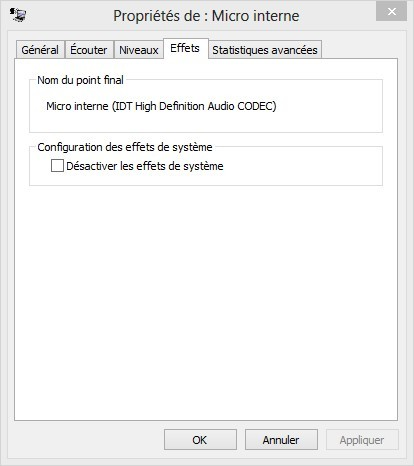
\includegraphics[scale=0.52]{images/win8config2} 
\end{tabular}
\end{center}

Pour Windows7, on fait le même test, le résultat est figuré ci-dessous:

\begin{center}
\begin{tabular}{c c}
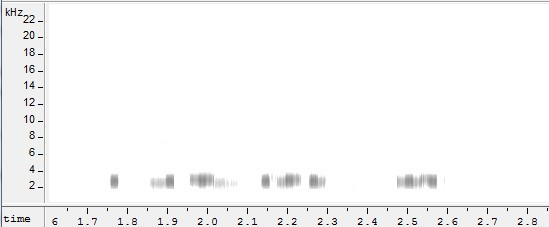
\includegraphics[scale=0.66]{images/Windows7Filtre} & 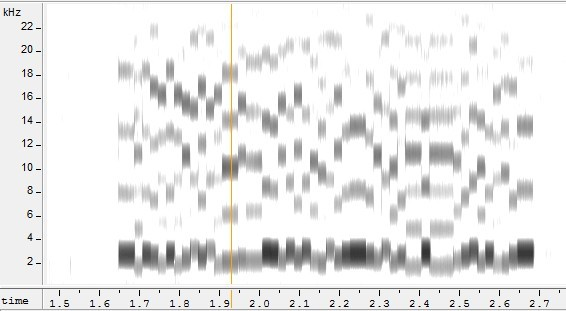
\includegraphics[scale=0.48]{images/Windows7Unfiltre} \\
Avec filtrage & Sans filtrage
\end{tabular}
\end{center}

Avec les configurations suivantes:
\begin{center}
\begin{tabular}{c c}
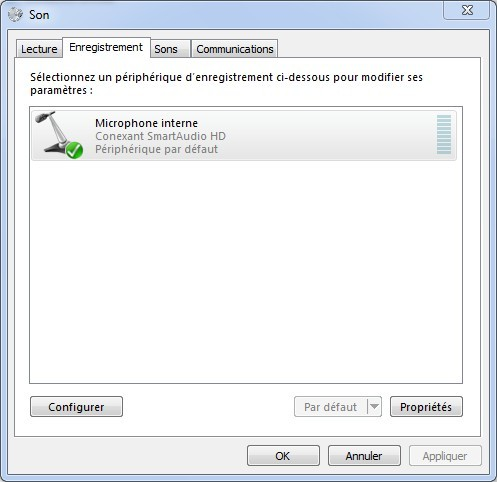
\includegraphics[scale=0.5]{images/Win7Config1} & 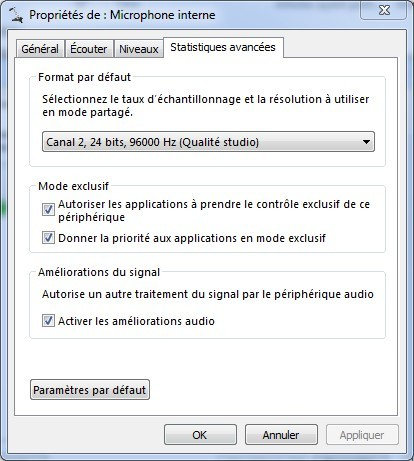
\includegraphics[scale=0.52]{images/Win7Config2} 
\end{tabular}
\end{center}

On peut voir que ce filtrage coupe les fréquences à partir de 4kHz environs.


\subsubsection{Les autres analyses}

J'ai aussi fait les autres analyses suivantes qui ne sont pas détaillés dans ce rapport:\\

\begin{itemize}
\item Analyse de volume de son par sonomètre
\item Différences entre les prototypes et les cartes
\item Analyse de l'effet environnement
\item etc...
\end{itemize}


